%!TEX root = skripsi.tex
%-----------------------------------------------------------------------------%
\chapter{\babTiga}
%-----------------------------------------------------------------------------%
%-----------------------------------------------------------------------------%
\section{Rancangan Sistem}
%-----------------------------------------------------------------------------%
% Ide, model matematik, rumus, fitur, jangan m=ngomongin teknologi (java, keras, dll), word2vec boleh %
Sistem yang akan \saya~buat dalam penelitian ini sesuai dengan rancangan arsitektur sistem pada gambar \ref{fig:arsitektur_sistem}.
\begin{figure}
  \centering
  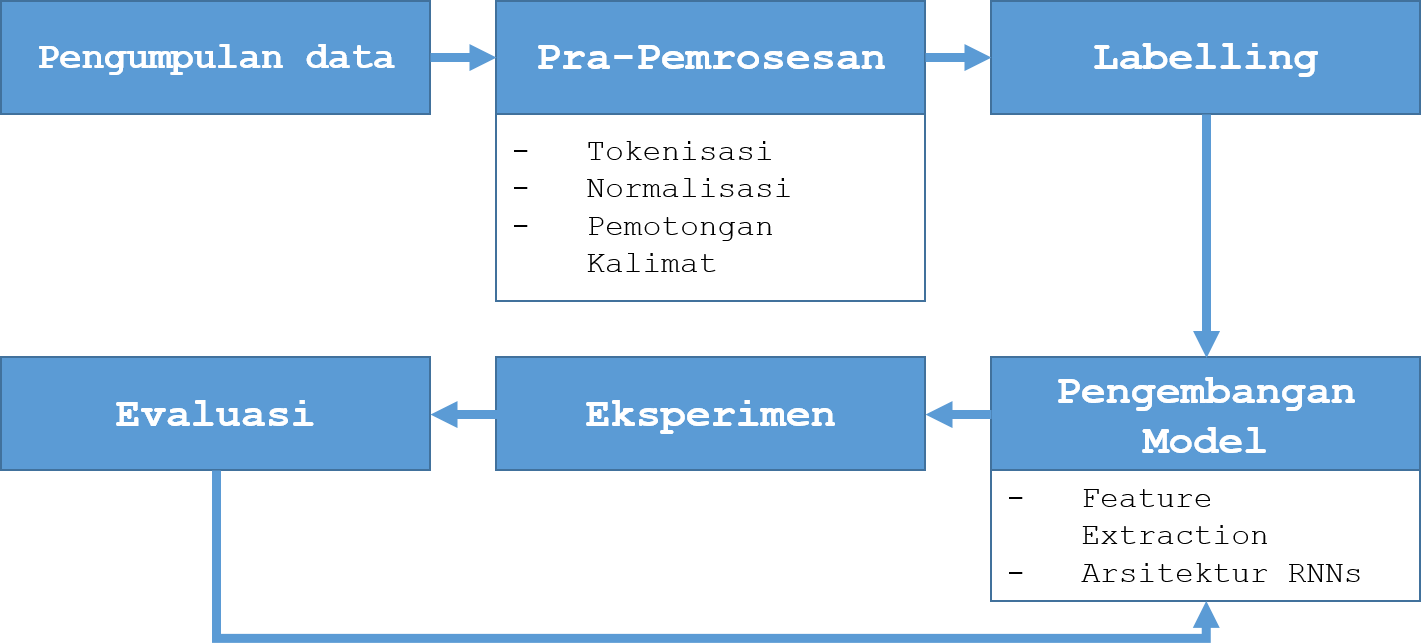
\includegraphics[width=\linewidth]{images/arsitektur}
  \caption{Rancangan Arsitektur Sistem}
  \label{fig:arsitektur_sistem}
\end{figure}

Berikut merupakan penjelasan alur dalam rancangan arsitektur sistem.
	\subsection{Pengumpulan Data}
	Pengumpulan data dilakukan dengan tujuan untuk mendapatkan data \textit{training} dan \textit{testing} sebagai \textit{input} sistem \mer~yang diusulkan. Data yang dimaksud merupakan teks dari forum kesehatan \textit{online} dari berbagai sumber. 
	
	\subsection{Pra-Pemrosesan}
	Pra-pemrosesan dilakukan dengan tujuan supaya teks yang diberikan mampu dibaca oleh sistem \mer. Dalam tahap ini, ada dua pekerjaan utama yang perlu dilakukan, yaitu:
	\begin{enumerate}
		\item Pembersihan data\\
		Langkah ini dilakukan dengan tujuan untuk membersihkan dokumen dari berbagai karakter yang tidak terdapat dalam karakter ASCII. Selain itu, perlu juga pengubahan beberapa tanda baca/token menjadi 1 token tersendiri. Misalnya sebuah token tautan (\textit{www.alodokter.com/asma/pengobatan}) diganti menjadi token "url".
		\item Tokenisasi\\
		Tokenisasi dilakukan untuk mendapatkan token yang paling tepat sebagai satu buah kata. Hal ini perlu dilakukan untuk menghindari beberapa kelompok token berbeda yang tergabung. Misalnya karakter abjad dengan karakter angka atau karakter abjad dengan karakter tanda baca dipisahkan berdasarkan kelompoknya.
		\item Pemotongan kalimat\\
		Untuk menghindari jumlah token yang timpang dalam kalimat yang berbeda dan data yang \textit{sparse}, diperlukan pemotongan kata yang tepat. Langkah-langkah yang diperlukan untuk melakukan pemotongan kata yaitu:
		\begin{enumerate}
			\item memisahkan kalimat berdasarkan tanda baca (.!?,),
			\item apabila suatu kalimat memiliki jumlah kata yang sedikit (misal diberikan batasan minimal 10 kata dalam satu kalimat), kalimat tersebut digabungkan dengan kalimat setelahnya.
		\end{enumerate}
	\end{enumerate}
	
	\subsection{Pelabelan}
	Pada tahap ini, \saya~melakukan pelabelan pada dokumen teks yang merupakan hasil pada tahap sebelumnya dengan label \disease, \symptom, \drug~dan \treatment. Berikut merupakan penjelasan dari masing-masing label:
	\begin{enumerate}
		\item \Disease\\
		Entitas \disease~yang dimaksud pada penelitian ini yaitu nama dari suatu penyakit. Penyakit merupakan keadaan abnormal yang timbul pada tubuh manusia. Contoh dari entitas \disease~yaitu:
		\begin{description}
			\item[$\bullet$] Skizofrenia
			\item[$\bullet$] Trikotilomania
			\item[$\bullet$] Diabetes melitus
		\end{description}
	
		\item \Symptom\\
		Entitas \symptom~yang dimaksud pada penelitian ini yaitu fenomena yang dialami oleh seseorang yang terkena suatu penyakit. Contoh dari entitas \symptom~yaitu:
		\begin{description}
			\item[$\bullet$] Napas berbunyi
			\item[$\bullet$] Benjolan di daerah perut
			\item[$\bullet$] Nyeri saat BAK
		\end{description}
	
		\item \Drug\\
		Entitas \drug~merupakan entitas nama obat dari suatu penyakit yang memiliki fungsi untuk mengurangi atau menyembuhkan penyakit tersebut. Contoh dari entitas \drug~yaitu:
		\begin{description}
			\item[$\bullet$] Paracetamol
			\item[$\bullet$] Diltiazem
			\item[$\bullet$] eritropoetin-alfa
		\end{description}
	
		\item \Treatment\\
		Entitas \treatment~merupakan cara atau langkah penyembuhan dari suatu penyakit. Contoh dari entitas \treatment~yaitu:
		\begin{description}
			\item[$\bullet$] Pemeriksaan darah rutin
			\item[$\bullet$] Penilaian denyut kapiler
			\item[$\bullet$] Terapi inhalasi
		\end{description}
	\end{enumerate}
		
	\subsection{Pengembangan Model}
	Pada tahap ini, \saya~melakukan pengusulan dan perancangan model yang nantinya akan \saya~evaluasi pada tahap eksperimen. Dalam mengembangkan model, terdapat dua pekerjaan yang\saya~lakukan, yaitu:
	
	\subsubsection{Ekstrasi Fitur}
	Pada tahap ini, \saya~melakukan ekstraksi fitur dari dokumen yang telah diberi label entitas. Ada beberapa fitur yang \saya~usulkan dalam penelitian ini yang nantinya \saya~kombinasikan supaya mendapatkan hasil terbaik. Fitur-fitur tersebut yaitu:
	\begin{enumerate}
		\item Fitur 1: Kata itu sendiri\\
		Fitur ini merupakan fitur kata dalam representasi vektor. Untuk mendapatkan representasi vektor dari masing-masing kata, penulis menggunakan \textit{word embedding}. Terdapat beberapa langkah yang perlu \saya~lakukan dalam memanfaatkan \textit{word embedding} ini, yaitu:
		\begin{enumerate}
			\item Pengumpulan data \textit{training} untuk \textit{word embedding}
			\item \textit{Training} untuk mendapatkan model \textit{word embedding}
			\item Pengubahan kata menjadi vektor dari model yang didapatkan
		\end{enumerate}
		
		\item Fitur 2: \textit{Part of Speech Tag} (POS-Tag)\\
		Fitur ini merupakan fitur \textit{tag} yang dimiliki setiap kata yang diusulkan oleh \cite{abacha2011medical} dalam penelitiannya di bidang \mer. Model yang digunakan merupakan model POS-Tag berbahasa Indonesia.
		
		\item Fitur 3: \textit{Stopword}\\
		Fitur ini merupakan fitur yang berisi vektor suatu kata merupakan \textit{stopword} atau bukan.
		
		\item Fitur 4: Kamus kesehatan\\
		Fitur kamus kata merupakan fitur yang berisi informasi suatu kata terdapat di dalam kamus kesehatan atau tidak. Pada penelitian ini, kamus kesehatan yang dipakai ada sejumlah entitas yang akan dikenali, yaitu kamus \disease, kamus \symptom, kamus \drug~dan kamus \treatment.\
		
		\item Fitur 5: Frasa kata benda\\
		Menurut \cite{hs2005bahasa}, frasa kata benda sendiri merupakan kelompok kata benda yang dibentuk dengan memperluas kata benda ke sekelilingnya. Fitur frasa kata benda yang \saya~gunakan dalam penelitian merupakan fitur yang berisi informasi suatu kata atau kumpulan kata merupakan frasa kata benda atau bukan. Dalam menentukan suatu kata merupakan frasa atau bukan, penulis menggunakan aturan pembentukan frasa yang digunakan pada bahasa Indonesia, yaitu:
		\begin{description}
		 	\item[$\bullet$] NP : NN
		 	\item[$\bullet$] NP : NNP
		 	\item[$\bullet$] NP : PR
		 	\item[$\bullet$] NP : PRP
		 	\item[$\bullet$] NP : NN + NN
		 	\item[$\bullet$] NP : NN + NNP
		 	\item[$\bullet$] NP : NN + PR
		 	\item[$\bullet$] NP : NN + PRP
		 	\item[$\bullet$] NP : NN + JJ
		 	\item[$\bullet$] NP : DT + NN
		 	\item[$\bullet$] NP : RB + NN
		 	\item[$\bullet$] NP : CD + NN
		 	\item[$\bullet$] NP : NND + NN
		 \end{description}
	 
		 \item Fitur 6: Frasa verbal\\
		 Menurut \cite{hs2005bahasa}, frasa verbal merupakan kelompok kata benda yang dibentuk dengan mkata kerja. Fitur frasa verbal yang \saya~gunakan dalam penelitian merupakan fitur yang berisi informasi suatu kata atau kumpulan kata merupakan frasa verbal atau bukan. Dalam menentukan suatu kata merupakan frasa atau bukan, penulis menggunakan aturan pembentukan frasa yang digunakan pada bahasa Indonesia, yaitu:
		 \begin{description}
		 	\item[$\bullet$] VP : VB
		 	\item[$\bullet$] VP : VB + NP
		 \end{description}
	 
		 \item Fitur 7: 1 kata sebelum
		 Fitur ini merupakan fitur yang berisi informasi kata sebelum kata saat ini yang direpresentasikan dalam bentuk vektor untuk masing-masing kata.
		 
		 \item Fitur 8: 1 kata sesudah
		 Fitur ini merupakan fitur yang berisi informasi kata sesudah kata saat ini yang direpresentasikan dalam bentuk vektor untuk masing-masing kata.
		 
		 \item Fitur 9: 2 kata sebelum
		 Fitur ini merupakan fitur yang berisi informasi 2 kata sebelum kata saat ini yang direpresentasikan dalam bentuk vektor untuk masing-masing kata.
		 
	\end{enumerate}

	\subsubsection{Pengusulan Arsitektur RNNs}
	Pada tahap ini \saya~mengusulkan arsitektur RNNs yang akan digunakan pada tahap eksperimen. Ada dua arsitektur yang \saya~gunakan dalam penelitian ini, yaitu
	\begin{enumerate}
		\item LSTM 1 layer\\
		Pada LSTM 1 layer, semua fitur yang menjadi input digabung menjadi satu. Misalnya .... Berikut merupakan ilustrasi LSTM 1 layer yang \saya~gunakan dalam penelitian ini.
		\item LSTM layer bertingkat
		Pada LSTM 2 layer, penulis mendefinisikan 2 layer, dimana layer terbawah merupakan layer dengan jumlah LSTM sebanyak n kelompok fitur. Pertama-tama fitur dikelompokkan terlebih dahulu, kemudian dijadikan input untuk LSTM layer pertama. Setelah itu, hasil dari layer pertama tersebut akan digabung menjadi satu, dengan menggunakan layer penggabung. \textit{Output} dari layer penggabung kemudian dimasukkan ke dalam LSTM layer kedua, yang \textit{output}-nya merupakan hasil klasifikasi label. Berikut merupakan ilustrasi dari LSTM layer bertingkat yang \saya~gunakan.
	\end{enumerate}
	
	\subsection{Eksperimen}
	Dalam melakukan eksperimen, arsitektur \textit{deep learning} yang \saya~gunakan ada;ah \textit{Recurrent Neural Networks}, dalam hal ini \saya~menggunakan LSTM. Hal ini \saya~lakukan karena pada penelitian \cite{mujiono2016new}, LSTM memberikan \textit{output} terbaik dalam \mer~yang dirancang. Selain itu, LSTM juga sangat baik dalam masalah \textit{sequence labelling} seperti yang dilakukan oleh \cite{graves2013speech} dan merupakan \textit{state-of-the-art} dalam bidang ini. Masih banyak penelitian lain yang membuktikan bahwa LSTM merupakan arsitektur \textit{deep learning} yang sangat baik dalam masalah \textit{sequence labelling} seperti \textit{Offline Hadwriting Recognition} \citep{graves2009offline}, \textit{sequence tagging} \citep{huang2015bidirectional}, \textit{Sequence to Sequence Learning} \citep{NIPS2014_5346} dan lain lain.
	
	Eksperimen yang \saya~lakukan menggunakan 10-\textit{cross fold validation}, karena keterbatasan data \textit{training} yang \saya~miliki. Sebelum melakukan eksperimen, \saya~membagi data \textit{training} menjadi 10 bagian, kemudian melakukan iterasi sebanyak 10 kali dimana pada masing-masing iterasi ke-i, bagian data ke-i menjadi data \textit{testing} dan yang lainnya digabung menjadi data \textit{training}. 
	
	Setelah melakukan pembagian dan pengelompokan data berdasarkan nomor iterasi, penulis membuat model dari data \textit{training} tersebut. Setelah \saya~mendapatkan model, \saya~melakukan testing terhadap masing-masing model dengan data \textit{testing} yang telah disediakan sebelumnya. Hasil dari pelabelan data \textit{testing} ini akan \saya~evaluasi di tahap selanjutnya. Setelah itu \saya~kembali melakukan pembuatan model dengan fitur yang berbeda, atau dengan tambahan fitur lain. Dalam perjalanan melakukan pengujian, apabila fitur yang diuji memberikan hasil yang bagus atau menambah akurasi, \saya~menggabungkan fitur ini ke percobaan selanjutnya. Namun apabila fitur pada saat ini memberikan akurasi yang lebih jelek, \saya~tidak menggunakan fitur tersebut di percobaan selanjutnya.
	
	\subsection{Evaluasi}
	Pada tahap ini, \saya~melakukan serangkaian evaluasi dari data \textit{testing} yang telah dilabeli dengan model yang dihasilkan pada tahap eksperimen. \Saya~melakukan evaluasi dengan menggunakan metode \textit{partial evaluation} dengan aturan sebagai berikut:
	
	\begin{enumerate}
		\item 
	\end{enumerate}
	
	
	Dalam melakukan evaluasi, \saya~menghitung \textit{f-measure}, \textit{precission} dan \textit{recall} untuk masing-masing entitas yang kemudian akan dihitung rata-ratanya baik dari masing-masing entitas maupun rata-rata keseluruhan. Angka-angka hasil evaluasi ini akan menjadi pertimbangan untuk penggunaan fitur pada saat ini di eksperimen selanjutnya. Apabila akurasi dari penggunaan fitur saat ini lebih baik atau meningkat dari eksperimen sebelumnya, \saya~menggunakan fitur ini pada eksperimen selanjutnya. Selain itu, \saya~juga mengevaluasi arsitektur RNNs yang \saya~gunakan.
	